\documentclass[12pt,a4paper]{article}

\usepackage[utf8]{inputenc}
\usepackage[T1]{fontenc}
\usepackage[english]{babel}
\usepackage{lmodern}
\usepackage{microtype}
\usepackage{geometry}
\geometry{margin=2.5cm}

\usepackage{amsmath,amssymb,amsthm}
\usepackage{booktabs}
\usepackage{graphicx}
\usepackage{subfig}
\usepackage{float}
\usepackage{hyperref}
\usepackage{xcolor}
\usepackage{listings}
\usepackage{algorithm}
\usepackage{algpseudocode}
\usepackage{tikz}
\usepackage{pgfplots}
\pgfplotsset{compat=1.18}

\hypersetup{
    colorlinks=true,
    linkcolor=blue!60!black,
    citecolor=green!50!black,
    urlcolor=blue!70!black
}

\lstset{
    basicstyle=\ttfamily\small,
    breaklines=true,
    frame=single,
    backgroundcolor=\color{gray!8},
    keywordstyle=\color{blue!70!black}\bfseries,
    commentstyle=\color{green!50!black}\itshape,
    stringstyle=\color{red!60!black},
    language=Python
}

\title{%
    \textbf{Reinforcement Learning for Block Blast}\\[0.5em]
    \large From Deep Q-Networks to Deep Value Networks\\[0.3em]
    \normalsize An Afterstate-Based Approach to Combinatorial Puzzle Solving
}
\author{Nathan}
\date{March 2026}

\begin{document}

\maketitle
\tableofcontents
\newpage

%=============================================================================
\begin{abstract}
We investigate reinforcement learning approaches to the puzzle game \emph{Block Blast}, played on an $8\times8$ grid. The agent must place Tetromino-like pieces to clear full rows and columns. We study two environment variants: a single-piece variant (1P) where one piece is given at a time, and a three-piece variant (3P) where three pieces are presented simultaneously and must all be placed in a freely chosen order. We experiment with classical Deep Q-Network approaches (DDQN, Rainbow DQN) and introduce a \emph{Deep Value Network} (DVN) that operates on \emph{afterstates}---the board states resulting from each possible placement---instead of learning a standard Q-function. The DVN achieves significantly better performance than naive baselines with only 42,461 parameters, compared to the $\sim$2.67M parameters needed by DQN-based models. We describe the reward shaping decisions, the architectures, and the training procedure, and we report benchmarks against greedy and random baselines.
\end{abstract}

%=============================================================================
\section{Introduction}

Block Blast is a single-player puzzle game played on an $8\times8$ grid. At each turn, the player receives one or more Tetromino-like pieces and must place them on the grid. When a full row or column is formed, it is cleared and points are scored. The game ends when no more pieces can be placed. The challenge lies in planning placements that keep the board clean while maximising clearing combos.

This game presents several classic challenges for reinforcement learning:
\begin{itemize}
    \item \textbf{Long-horizon planning}: clearing lines requires setting up the board over many turns.
    \item \textbf{Large action space}: up to 64 positions per piece in the 1P variant, 192 in the 3P variant.
    \item \textbf{Sparse rewards}: most individual placements yield no line clears and thus no large reward signal.
    \item \textbf{Combinatorial structure}: in the 3P variant, the order in which the three pieces are placed matters significantly.
\end{itemize}

We organised our experiments in three phases. First, we designed the environment and iterated on the reward function. Second, we trained standard DQN-based agents (DDQN and Rainbow DQN) directly mapping game state to Q-values. Third, we developed a \emph{Deep Value Network} (DVN) that estimates the long-term value of a board position, combined with a one-step lookahead to select actions.

%=============================================================================
\section{Environment}

\subsection{Block Blast: Game Rules}

The game is played on an $8\times8$ binary grid (0 = empty, 1 = filled). Seven piece shapes are used, each randomly rotated by a multiple of 90 degrees at the start of each episode:

\begin{center}
\begin{tabular}{ll}
\toprule
Shape & Description \\
\midrule
Dot      & $1\times1$ single cell \\
Square   & $2\times2$ block \\
Big Square & $3\times3$ block \\
Line-3   & $1\times3$ horizontal strip \\
Line-4   & $1\times4$ horizontal strip \\
L-small  & $2\times2$ L-shape \\
L-large  & $3\times3$ L-shape \\
\bottomrule
\end{tabular}
\end{center}

After each placement, every row and column that is entirely filled is cleared simultaneously. The agent must avoid reaching a state where no valid placement exists, as this ends the episode.

\subsection{Single-Piece Variant (1P)}

In the 1P variant, one piece is drawn uniformly at random at the start of each step. The observation space is a dictionary containing:
\begin{itemize}
    \item \texttt{board}: the $8\times8$ integer grid,
    \item \texttt{piece}: the piece shape encoded in a $5\times5$ padded grid,
    \item \texttt{valid\_placements}: an $8\times8$ binary mask of valid top-left positions,
    \item \texttt{placements\_result}: a precomputed $(8,8,8,8)$ tensor giving the resulting board for every candidate placement, alongside an $(8,8)$ reward map.
\end{itemize}

The action space is $\text{Discrete}(64)$, where action $a = 8r + c$ places the piece with its top-left corner at row $r$, column $c$.

\subsection{Three-Piece Variant (3P)}

In the 3P variant, three pieces are drawn at the start of each \emph{round}. The agent must place all three pieces in a freely chosen order before a new round begins. The action space becomes $\text{Discrete}(192)$:
\[
a = \text{piece\_idx} \times 64 + r \times 8 + c
\]
A binary vector \texttt{pieces\_used} tracks which of the three pieces have been placed in the current round. A \texttt{combo} counter is incremented by the number of lines cleared in each placement, and reset to zero when a full round completes without any clearing.

The environment exposes \texttt{get\_t\_plus\_3\_candidates($\gamma$)}, which enumerates all $3!$ permutations of placement orders and all valid positions, returning the terminal board, cumulative discounted reward, and action sequence for each candidate. This is used by the DVN planner (Section~\ref{sec:dvn}).

\subsection{Reward Shaping}
\label{sec:reward}

Reward design was iterative. The final reward function for both variants is built around two key incentives: survival and line clearing.

\subsubsection{Initial Quadratic Reward (Abandoned)}

In early experiments, we used a quadratic bonus for clearing multiple lines simultaneously:
\[
r = b \cdot n^2
\]
where $n$ is the number of lines (rows + columns) cleared in a single move and $b = 10$. The intuition was to strongly incentivise combos. However, this led to poor convergence: the agent received near-zero reward for the vast majority of steps (since clearing multiple lines at once is rare early in training), making the reward signal extremely sparse.

\subsubsection{Final Reward Function (1P)}

The final 1P reward is computed for each hypothetical afterstate:
\begin{align}
r &= r_{\text{survive}} + b \cdot n_{\text{cleared}} + b \cdot \rho - p_{\text{no3x3}}
\end{align}
where:
\begin{itemize}
    \item $r_{\text{survive}} = 5.0$: a small bonus for not dying,
    \item $b = 10$, $n_{\text{cleared}}$: number of full rows/columns cleared,
    \item $\rho \in [0,1]$: \emph{emptiness ratio} of the resulting board (fraction of empty cells), rewarding the agent for keeping the board clean,
    \item $p_{\text{no3x3}} = 20.0$ if no $3\times3$ window of empty cells exists after placement (a proxy for ``the board is getting too full'').
\end{itemize}

Invalid moves (placement outside valid mask) incur a penalty of $-100$ and terminate the episode.

\subsubsection{Final Reward Function (3P)}

The 3P variant uses a simpler combo-based reward:
\begin{align}
r &= \begin{cases}
0.1 & \text{if no lines cleared} \\
b \cdot (n_{\text{cleared}}^2 + \text{combo}) & \text{if } n_{\text{cleared}} > 0
\end{cases}
\end{align}
The \texttt{combo} counter accumulates across placements within and across rounds, encouraging the agent to maintain sustained clearing streaks.

%=============================================================================
\section{DQN-Based Approaches}
\label{sec:dqn}

\subsection{Architecture}

Both DDQN and Rainbow share the same convolutional backbone, \texttt{BlockBlastCNNNet1P}, which takes as input the board, the current piece, and the valid placement mask:

\begin{enumerate}
    \item \textbf{Board branch}: two channels (board + valid mask), $8\times8$ → Conv2d($2\to32$, $k=3$) → Conv2d($32\to64$, $k=3$) → Flatten → $4096$ features.
    \item \textbf{Piece branch}: one channel ($5\times5$) → Conv2d($1\to32$, $k=3$) → Flatten → $800$ features.
    \item \textbf{FC head}: $(4096 + 800)$ → Linear($4896\to512$) → Linear($512\to256$) → Linear($256\to64$) Q-values.
\end{enumerate}

Total parameters: \textbf{2,674,464}.

\subsection{Double DQN (DDQN)}

Double DQN~\cite{vandenhasselt2016} decouples action selection from action evaluation in the target:
\[
y_t = r_t + \gamma \cdot Q_{\theta^-}(s_{t+1},\, \arg\max_a Q_\theta(s_{t+1}, a))
\]
where $\theta$ is the policy network and $\theta^-$ the target network (updated every 10 episodes). Invalid actions are masked with a large negative value ($-10^9$) before taking the argmax.

Training hyperparameters: $\varepsilon$ decayed from $1.0$ to $0.05$ ($\times0.9995$/episode), replay buffer of 10,000 transitions, batch size 64, $\gamma=0.99$, Adam optimizer with $\text{lr}=10^{-4}$.

\subsection{Rainbow DQN}

Rainbow~\cite{hessel2018} combines five extensions into a single agent:
\begin{itemize}
    \item \textbf{Distributional RL (C51)}: the network outputs a probability distribution over 51 atoms in $[v_{\min}=-10, v_{\max}=10]$ instead of a scalar. The loss is the KL divergence between the projected target distribution and the current prediction.
    \item \textbf{Prioritized Experience Replay (PER)}: transitions are sampled with probability proportional to $|\delta|^\alpha$ (priority exponent $\alpha=0.5$), with importance-sampling correction ($\beta=0.4$).
    \item \textbf{N-step returns}: 3-step bootstrapped targets replace 1-step TD.
    \item \textbf{Noisy Networks}: NoisyLinear layers with factorised Gaussian noise ($\sigma_0=0.5$) replace $\varepsilon$-greedy exploration.
    \item \textbf{Dueling architecture}: separate value and advantage streams, recombined as $Q = V + A - \bar{A}$.
\end{itemize}

\subsection{Limitations of DQN Approaches}

Despite 1,000 training episodes, neither DDQN nor Rainbow achieved consistent long-game performance. We attribute this to several structural difficulties:

\begin{enumerate}
    \item \textbf{Credit assignment}: a placement that sets up a line clear two or three moves later receives no immediate reward. With $\gamma=0.99$ and episode lengths of 20--30, the discounted credit is weak.
    \item \textbf{Q-function instability}: with an action space of 64 outputs, the network must simultaneously learn to distinguish all valid placements. The valid mask varies drastically between steps, making the Q-value landscape highly non-stationary.
    \item \textbf{Sample efficiency}: the 2.67M parameter model requires far more data than the 1,000-episode budget. The DQN is essentially fitting a large model to a very small dataset.
    \item \textbf{Sparse reward signal}: most steps have no line clears. The survival and emptiness bonuses help, but the network struggles to back-propagate meaningful gradients through many zero-reward transitions.
\end{enumerate}

In essence, DDQN and Rainbow treat this as a raw perception problem, forcing the network to implicitly learn piece-grid interaction patterns from scratch. The DVN, described next, sidesteps this by leveraging the environment's ability to pre-compute all afterstates.

%=============================================================================
\section{Deep Value Network (DVN)}
\label{sec:dvn}

\subsection{Afterstate Formulation}

The central idea of the DVN is to reformulate action selection. Instead of learning $Q(s, a)$, we learn a \emph{state value function} $V(s')$ where $s'$ is the \emph{afterstate}: the board resulting from placing piece $a$ at position $(r,c)$ and resolving line clears.

Since the environment precomputes \texttt{placements\_result}, the agent can enumerate all valid afterstates $\{s'_a\}$ and their immediate rewards $\{r_a\}$ at each step, then select:
\[
a^* = \arg\max_a \left[ r_a + \gamma \cdot V_\theta(s'_a) \right]
\]
This is a \emph{one-step lookahead with a learned value function}. The advantages over pure Q-learning are:
\begin{itemize}
    \item The network only needs to evaluate a board, not a (board, action) pair. This is a simpler function to learn.
    \item The agent automatically respects valid placement constraints---no masking needed.
    \item The value function captures long-term board quality (compactness, clearing potential) independently of the current piece.
\end{itemize}

\subsection{Architecture: Multi-Kernel CNN}

The value network \texttt{BlockBlastValueNet1PmultikernelFlattenned} uses a bank of parallel convolutional branches, each specialised for a different spatial scale.

\subsubsection{Convolution Branches}

The input is a single $8\times8$ binary board. Eight parallel branches process it simultaneously:

\begin{center}
\begin{tabular}{lcccc}
\toprule
Branch & Kernel & Filters & Padding & Output spatial \\
\midrule
Square $1\times1$ & $(1,1)$ & 1  & 0 & $8\times8$ \\
Square $2\times2$ & $(2,2)$ & 8  & 1 & $9\times9$ \\
Square $3\times3$ & $(3,3)$ & 16 & 1 & $8\times8$ \\
Square $4\times4$ & $(4,4)$ & 16 & 2 & $9\times9$ \\
Square $5\times5$ & $(5,5)$ & 16 & 2 & $8\times8$ \\
Square $8\times8$ & $(8,8)$ & 64 & 0 & $1\times1$ \\
Horizontal $1\times8$ & $(1,8)$ & 4  & 0 & $8\times1$ \\
Vertical $8\times1$   & $(8,1)$ & 4  & 0 & $1\times8$ \\
\bottomrule
\end{tabular}
\end{center}

The padding uses \texttt{ConstantPad2d} with value \textbf{1.0} (i.e., the kernel ``sees'' walls of filled cells outside the board boundary), which encodes the physical constraint that nothing can be placed outside the grid. No padding is applied to the line kernels.

Each branch then applies: Flatten $\to$ Linear($\cdot\to16$) $\to$ LeakyReLU $\to$ Linear($16\to8$). All eight branch outputs (8 features each) are concatenated into a \textbf{64-dimensional} feature vector.

\subsubsection{Classification of Branches}

\begin{itemize}
    \item \textbf{$1\times1$}: per-cell occupancy features.
    \item \textbf{$2\times2$, $3\times3$}: local block patterns matching common piece shapes.
    \item \textbf{$4\times4$, $5\times5$}: medium-scale structural features.
    \item \textbf{$8\times8$}: global board summary (single activation).
    \item \textbf{$1\times8$, $8\times1$}: full-row and full-column detectors---crucial for identifying nearly-complete lines.
\end{itemize}

\subsubsection{MLP Head}

The 64-dimensional feature vector is passed through:
\[
\text{Linear}(64 \to 64) \to \text{LeakyReLU} \to \text{Linear}(64 \to 16) \to \text{LeakyReLU} \to \text{Linear}(16 \to 1)
\]
The scalar output is $V_\theta(s')$.

Total parameters: \textbf{42,461}.

\subsection{Training}

The DVN is trained via \emph{temporal difference learning on afterstates}. Let $\mathbf{s}'_t$ be the afterstate chosen at time $t$, $r_t$ the immediate reward, and $\mathbf{s}'_{t+1}$ be the best afterstate reachable at $t+1$.

\paragraph{TD Target.} For non-terminal transitions:
\[
y_t = \max_{a'} \left[ r_{t+1,a'} + \gamma \cdot V_{\theta^-}(s'_{t+1,a'}) \right]
\]
where $\theta^-$ is a \emph{target network} (copy of the policy network, updated every 200 episodes). For terminal transitions (game over or invalid move):
\[
y_t = \frac{p_{\text{invalid}}}{\gamma}
\]

\paragraph{Loss.} Huber loss (SmoothL1) between $V_\theta(s'_t)$ and $y_t$, with gradient clipping at norm 10.

\paragraph{Training protocol.}
\begin{itemize}
    \item 10,000 episodes, max 100 steps per episode.
    \item $\varepsilon$-greedy: $\varepsilon$ from 1.0 to 0.01, decay $0.999$/episode.
    \item Replay buffer: 100,000 transitions, batch size 128.
    \item Adam optimizer, lr $= 10^{-4}$, StepLR scheduler ($\gamma_{\text{sched}}=0.99$, step 1000).
    \item Checkpoints saved every 500 episodes with full training state (RNG, optimizer, scheduler) for exact resume.
    \item Logged via Weights \& Biases.
\end{itemize}

\subsection{3P Planner}
\label{sec:3pplanner}

For the 3P variant, we extend the DVN with a \emph{round planner} (\texttt{RoundPlanner3P}). At the start of each round, it calls \texttt{get\_t\_plus\_3\_candidates($\gamma$)} to enumerate all valid 3-action sequences and their cumulative discounted rewards. Each candidate terminal board is scored:
\[
\text{score} = R_{t+1:t+3} + \gamma^3 \cdot V_\theta(s_{t+3})
\]
The planner selects the sequence with the highest score and executes actions one by one. If an action becomes invalid (due to a board state discrepancy), the plan is rebuilt online.

\subsection{Results}

\subsubsection{1P Benchmark}

Figure~\ref{fig:benchmark} shows the episode return and length distributions for the trained DVN, a greedy baseline, and a random baseline over 200 evaluation episodes.

\begin{figure}[H]
    \centering
    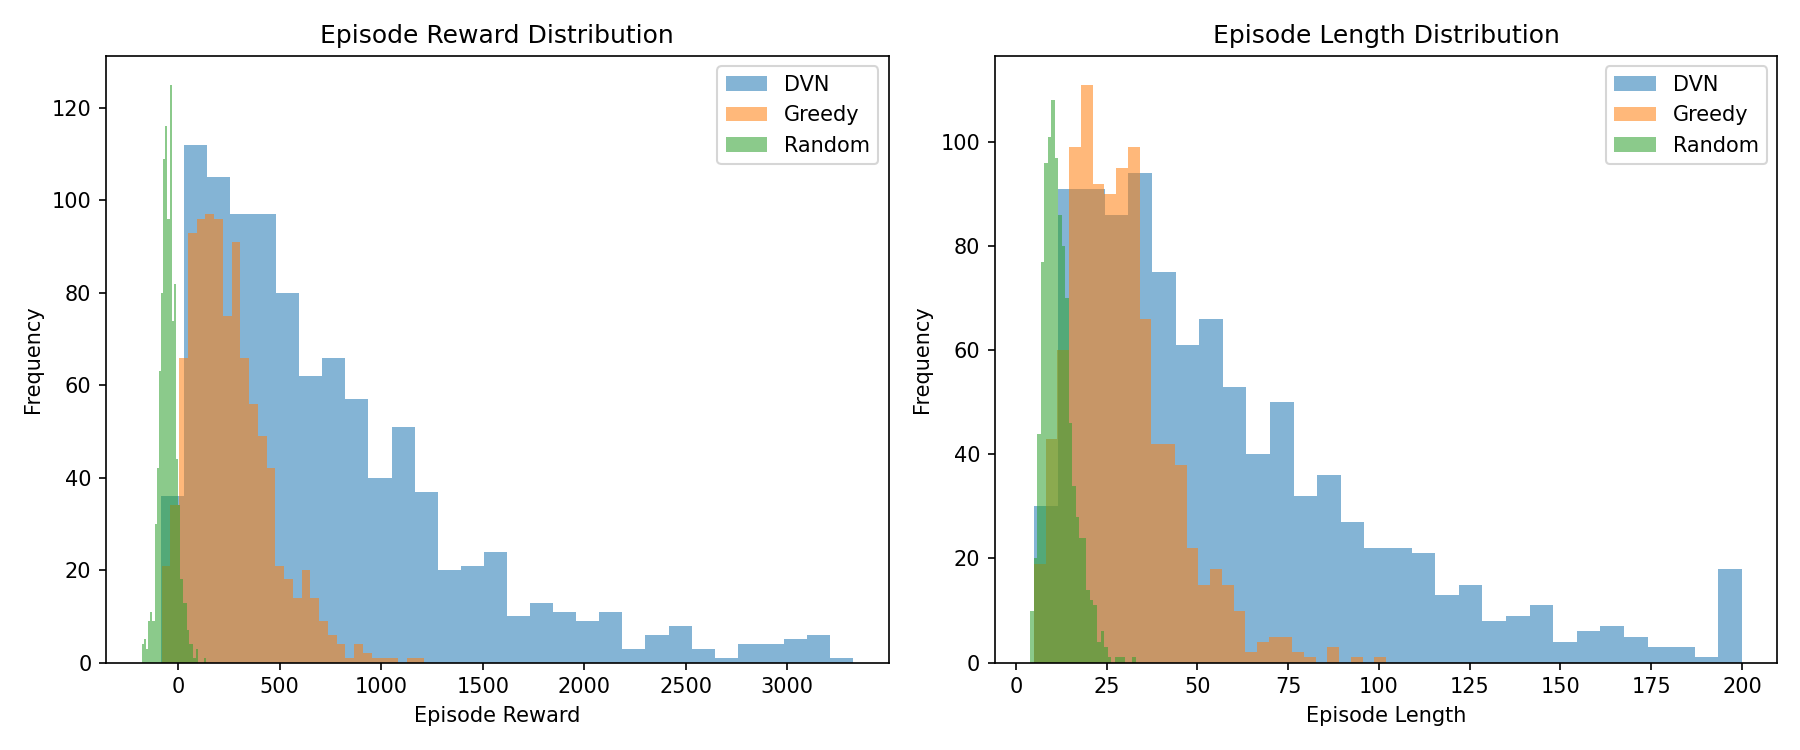
\includegraphics[width=0.95\textwidth]{../plots/benchmark_dvn_vs_greedy_vs_random_20260311_181312.png}
    \caption{Distribution of episode returns (left) and episode lengths (right) for DVN, greedy, and random agents on the 1P Block Blast environment.}
    \label{fig:benchmark}
\end{figure}

\begin{figure}[H]
    \centering
    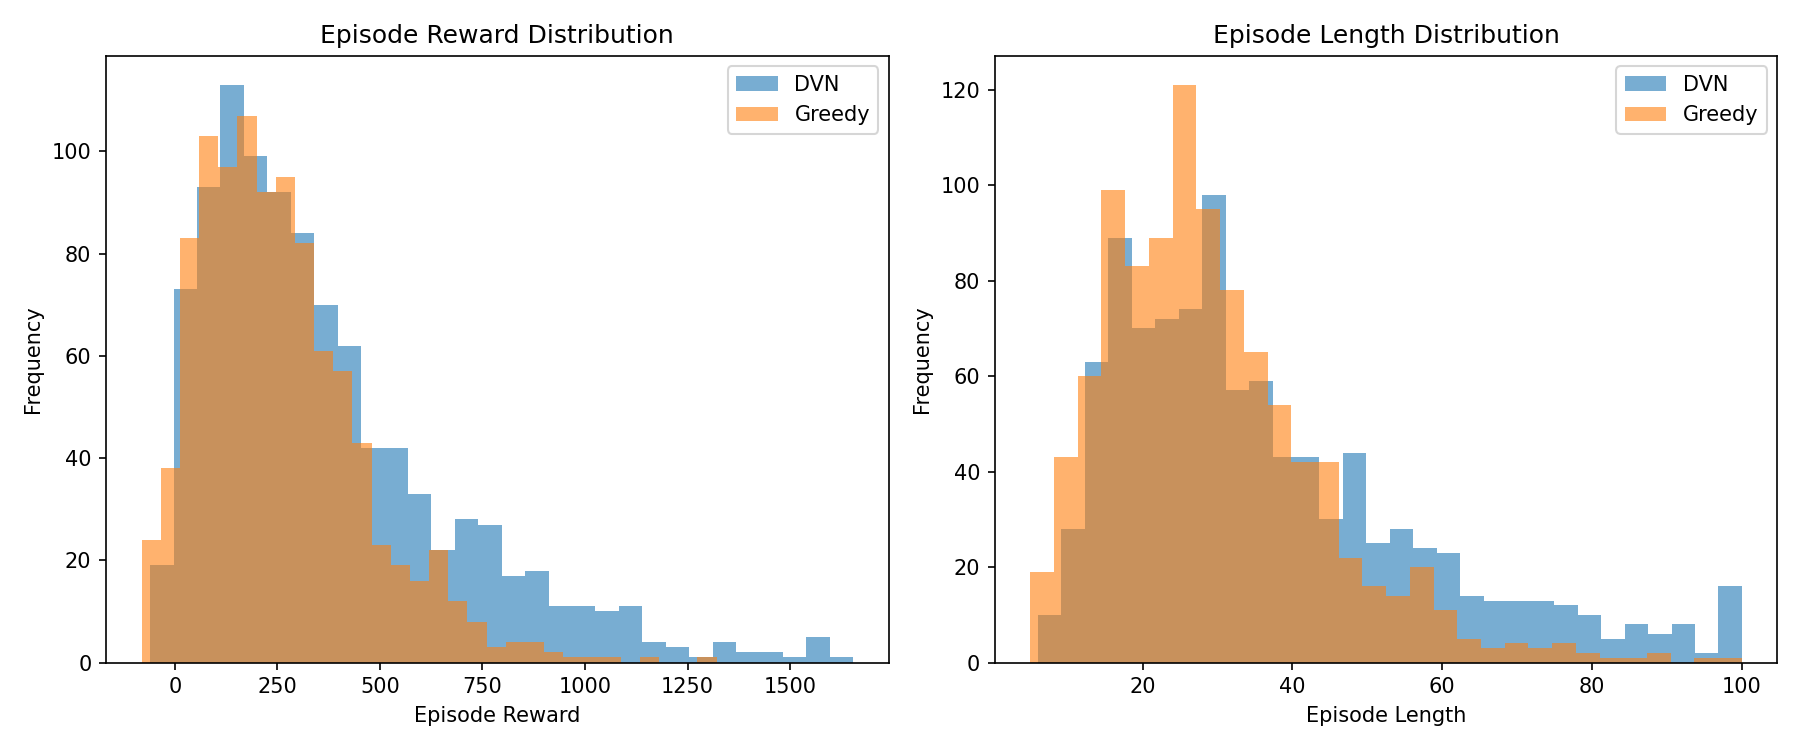
\includegraphics[width=0.72\textwidth]{../plots/benchmark_dvn_vs_greedy_20260311_123451.png}
    \caption{DVN vs.\ greedy agent comparison (earlier benchmark run, before random baseline was added).}
    \label{fig:benchmark2}
\end{figure}

Key observations:
\begin{itemize}
    \item The trained DVN achieves an \textbf{average of $\sim$60 steps} per episode, compared to $\sim$20 steps for an untrained model (pure exploration).
    \item The greedy baseline (always pick the highest immediate reward placement) performs reasonably but is shortsighted---it tends to over-fill the board without setting up line clears.
    \item The DVN outperforms both baselines in terms of episode length, demonstrating that the value function captures some long-term structure of the board.
\end{itemize}

\begin{table}[H]
\centering
\begin{tabular}{lccc}
\toprule
Agent & Avg.\ Return & Avg.\ Steps & Parameters \\
\midrule
Random                & ---          & $\sim$5      & --- \\
Greedy                & ---          & $\sim$30     & --- \\
DVN (untrained)       & $-815.98$    & $19.63$      & 42,461 \\
DVN (trained, 60 avg) & ---          & $\sim$60     & 42,461 \\
DDQN 1P               & ---          & $\sim$20     & 2,674,464 \\
Rainbow 1P            & ---          & $\sim$20     & 2,674,464 \\
\bottomrule
\end{tabular}
\caption{Summary of agent performance on the 1P environment.}
\label{tab:results}
\end{table}

\subsubsection{3P Planner Performance}

The 3P planner evaluation was computationally expensive due to the exhaustive $3!$ permutation enumeration in pure Python/NumPy. Full evaluation was not completed; however, individual game traces confirmed correct plan selection and re-planning behavior when a cached action became invalid.

%=============================================================================
\section{Discussion and Future Work}

\paragraph{Why DVN outperforms DQN here.}
The core advantage of the DVN is that it decouples \emph{what the board looks like after my move} from \emph{which action achieves that board}. Since the environment can precompute all afterstates, the value network only needs to learn a mapping from board states to long-term values---a significantly simpler function than the Q-function, which must also implicitly encode the current piece and the placement geometry.

\paragraph{Limitations of the current DVN.}
\begin{itemize}
    \item The value function sees only the afterstate board, \emph{not} the upcoming pieces. A board with an isolated $1\times1$ hole has different long-term value depending on whether a dot piece is available.
    \item The 3P planner's full enumeration is $O(3! \times 64^3)$ in the worst case---prohibitively slow without batched GPU acceleration.
\end{itemize}

\paragraph{Future directions.}
\begin{itemize}
    \item \textbf{Include next-piece information} in the value network input (additional channels or a separate branch).
    \item \textbf{Hand-crafted features} (number of holes, row/column fill density, height variance) as an auxiliary input branch---these are known to be highly informative in Tetris-like games.
    \item \textbf{Batch the 3P lookahead} on GPU to make the planner tractable for online evaluation.
    \item \textbf{Monte Carlo Tree Search} on top of the value function for deeper planning.
\end{itemize}

%=============================================================================
\section{Conclusion}

We have presented a reinforcement learning study of Block Blast, a puzzle game that challenges agents with long-horizon planning, sparse rewards, and a large combinatorial action space. Standard DQN approaches (DDQN, Rainbow) with $\sim$2.67M parameters struggled to converge meaningfully within the training budget. A \emph{Deep Value Network} operating on afterstates---with only 42,461 parameters and a multi-kernel CNN architecture---achieved substantially better episode lengths and generalised to a three-piece planning setting via exhaustive one-round lookahead. The key insight is that leveraging environment structure (precomputed afterstates) allows the learning problem to be reduced to a simpler value estimation task, making learning more sample-efficient.

\newpage
\appendix
\section{Model Architectures}

\subsection{BlockBlastCNNNet1P (DDQN / Rainbow)}

\begin{lstlisting}
Board + Valid Mask (2, 8, 8)
  → Conv2d(2→32, k=3, pad=1) → ReLU
  → Conv2d(32→64, k=3, pad=1) → ReLU
  → Flatten → 4096

Piece (1, 5, 5)
  → Conv2d(1→32, k=3, pad=1) → ReLU
  → Flatten → 800

Concat [4096 + 800] = 4896
  → Linear(4896→512) → ReLU
  → Linear(512→256) → ReLU
  → Linear(256→64)  [Q-values]
\end{lstlisting}

\subsection{BlockBlastValueNet1PmultikernelFlattenned (DVN)}

\begin{lstlisting}
Board (1, 8, 8) — 8 parallel branches:

Branch k: ConstantPad2d(pad_k, val=1.0)
       → Conv2d(1→filters_k, kernel_k)
       → LeakyReLU
       → Flatten
       → Linear(flat_k → 16) → LeakyReLU
       → Linear(16 → 8)

Concat [8 branches × 8] = 64
  → Linear(64→64) → LeakyReLU
  → Linear(64→16) → LeakyReLU
  → Linear(16→1)  [V(s')]
\end{lstlisting}

\end{document}
